\documentclass[twoside]{book}

% Packages required by doxygen
\usepackage{fixltx2e}
\usepackage{calc}
\usepackage{doxygen}
\usepackage[export]{adjustbox} % also loads graphicx
\usepackage{graphicx}
\usepackage[utf8]{inputenc}
\usepackage{makeidx}
\usepackage{multicol}
\usepackage{multirow}
\PassOptionsToPackage{warn}{textcomp}
\usepackage{textcomp}
\usepackage[nointegrals]{wasysym}
\usepackage[table]{xcolor}

% Font selection
\usepackage[T1]{fontenc}
\usepackage[scaled=.90]{helvet}
\usepackage{courier}
\usepackage{amssymb}
\usepackage{sectsty}
\renewcommand{\familydefault}{\sfdefault}
\allsectionsfont{%
  \fontseries{bc}\selectfont%
  \color{darkgray}%
}
\renewcommand{\DoxyLabelFont}{%
  \fontseries{bc}\selectfont%
  \color{darkgray}%
}
\newcommand{\+}{\discretionary{\mbox{\scriptsize$\hookleftarrow$}}{}{}}

% Page & text layout
\usepackage{geometry}
\geometry{%
  a4paper,%
  top=2.5cm,%
  bottom=2.5cm,%
  left=2.5cm,%
  right=2.5cm%
}
\tolerance=750
\hfuzz=15pt
\hbadness=750
\setlength{\emergencystretch}{15pt}
\setlength{\parindent}{0cm}
\setlength{\parskip}{3ex plus 2ex minus 2ex}
\makeatletter
\renewcommand{\paragraph}{%
  \@startsection{paragraph}{4}{0ex}{-1.0ex}{1.0ex}{%
    \normalfont\normalsize\bfseries\SS@parafont%
  }%
}
\renewcommand{\subparagraph}{%
  \@startsection{subparagraph}{5}{0ex}{-1.0ex}{1.0ex}{%
    \normalfont\normalsize\bfseries\SS@subparafont%
  }%
}
\makeatother

% Headers & footers
\usepackage{fancyhdr}
\pagestyle{fancyplain}
\fancyhead[LE]{\fancyplain{}{\bfseries\thepage}}
\fancyhead[CE]{\fancyplain{}{}}
\fancyhead[RE]{\fancyplain{}{\bfseries\leftmark}}
\fancyhead[LO]{\fancyplain{}{\bfseries\rightmark}}
\fancyhead[CO]{\fancyplain{}{}}
\fancyhead[RO]{\fancyplain{}{\bfseries\thepage}}
\fancyfoot[LE]{\fancyplain{}{}}
\fancyfoot[CE]{\fancyplain{}{}}
\fancyfoot[RE]{\fancyplain{}{\bfseries\scriptsize Generated by Doxygen }}
\fancyfoot[LO]{\fancyplain{}{\bfseries\scriptsize Generated by Doxygen }}
\fancyfoot[CO]{\fancyplain{}{}}
\fancyfoot[RO]{\fancyplain{}{}}
\renewcommand{\footrulewidth}{0.4pt}
\renewcommand{\chaptermark}[1]{%
  \markboth{#1}{}%
}
\renewcommand{\sectionmark}[1]{%
  \markright{\thesection\ #1}%
}

% Indices & bibliography
\usepackage{natbib}
\usepackage[titles]{tocloft}
\setcounter{tocdepth}{3}
\setcounter{secnumdepth}{5}
\makeindex

% Hyperlinks (required, but should be loaded last)
\usepackage{ifpdf}
\ifpdf
  \usepackage[pdftex,pagebackref=true]{hyperref}
\else
  \usepackage[ps2pdf,pagebackref=true]{hyperref}
\fi
\hypersetup{%
  colorlinks=true,%
  linkcolor=blue,%
  citecolor=blue,%
  unicode%
}

% Custom commands
\newcommand{\clearemptydoublepage}{%
  \newpage{\pagestyle{empty}\cleardoublepage}%
}

\usepackage{caption}
\captionsetup{labelsep=space,justification=centering,font={bf},singlelinecheck=off,skip=4pt,position=top}

%===== C O N T E N T S =====

\begin{document}

% Titlepage & ToC
\hypersetup{pageanchor=false,
             bookmarksnumbered=true,
             pdfencoding=unicode
            }
\pagenumbering{alph}
\begin{titlepage}
\vspace*{7cm}
\begin{center}%
{\Large Nogame \\[1ex]\large v1.\+1 }\\
\vspace*{1cm}
{\large Generated by Doxygen 1.8.13}\\
\end{center}
\end{titlepage}
\clearemptydoublepage
\pagenumbering{roman}
\tableofcontents
\clearemptydoublepage
\pagenumbering{arabic}
\hypersetup{pageanchor=true}

%--- Begin generated contents ---
\chapter{Hierarchical Index}
\section{Class Hierarchy}
This inheritance list is sorted roughly, but not completely, alphabetically\+:\begin{DoxyCompactList}
\item \contentsline{section}{Assets}{\pageref{class_assets}}{}
\item \contentsline{section}{image\+Loader}{\pageref{classimage_loader}}{}
\item \contentsline{section}{Locatie}{\pageref{class_locatie}}{}
\item \contentsline{section}{Main\+Frame}{\pageref{class_main_frame}}{}
\item \contentsline{section}{Richting}{\pageref{enum_richting}}{}
\item Runnable\begin{DoxyCompactList}
\item \contentsline{section}{Speelveld}{\pageref{class_speelveld}}{}
\end{DoxyCompactList}
\item \contentsline{section}{Tegel}{\pageref{class_tegel}}{}
\begin{DoxyCompactList}
\item \contentsline{section}{Doel}{\pageref{class_doel}}{}
\item \contentsline{section}{Leeg}{\pageref{class_leeg}}{}
\item \contentsline{section}{Muur}{\pageref{class_muur}}{}
\item \contentsline{section}{Speler}{\pageref{class_speler}}{}
\end{DoxyCompactList}
\item Key\+Listener\begin{DoxyCompactList}
\item \contentsline{section}{key\+Manager}{\pageref{classkey_manager}}{}
\end{DoxyCompactList}
\end{DoxyCompactList}

\chapter{Class Index}
\section{Class List}
Here are the classes, structs, unions and interfaces with brief descriptions\+:\begin{DoxyCompactList}
\item\contentsline{section}{\hyperlink{class_assets}{Assets} }{\pageref{class_assets}}{}
\item\contentsline{section}{\hyperlink{class_doel}{Doel} }{\pageref{class_doel}}{}
\item\contentsline{section}{\hyperlink{classimage_loader}{image\+Loader} }{\pageref{classimage_loader}}{}
\item\contentsline{section}{\hyperlink{classkey_manager}{key\+Manager} }{\pageref{classkey_manager}}{}
\item\contentsline{section}{\hyperlink{class_leeg}{Leeg} }{\pageref{class_leeg}}{}
\item\contentsline{section}{\hyperlink{class_locatie}{Locatie} }{\pageref{class_locatie}}{}
\item\contentsline{section}{\hyperlink{class_main_frame}{Main\+Frame} }{\pageref{class_main_frame}}{}
\item\contentsline{section}{\hyperlink{class_muur}{Muur} }{\pageref{class_muur}}{}
\item\contentsline{section}{\hyperlink{enum_richting}{Richting} }{\pageref{enum_richting}}{}
\item\contentsline{section}{\hyperlink{class_speelveld}{Speelveld} }{\pageref{class_speelveld}}{}
\item\contentsline{section}{\hyperlink{class_speler}{Speler} }{\pageref{class_speler}}{}
\item\contentsline{section}{\hyperlink{class_tegel}{Tegel} }{\pageref{class_tegel}}{}
\end{DoxyCompactList}

\chapter{Class Documentation}
\hypertarget{class_assets}{}\section{Assets Class Reference}
\label{class_assets}\index{Assets@{Assets}}
\subsection*{Static Public Member Functions}
\begin{DoxyCompactItemize}
\item 
static void \hyperlink{class_assets_a0c3276b3cea06ea62ae1362d98661124}{init} (int level)
\end{DoxyCompactItemize}
\subsection*{Static Public Attributes}
\begin{DoxyCompactItemize}
\item 
\mbox{\Hypertarget{class_assets_a81804b26e4d32ba4f1c0c94058e3b2f8}\label{class_assets_a81804b26e4d32ba4f1c0c94058e3b2f8}} 
static Buffered\+Image {\bfseries speler}
\item 
\mbox{\Hypertarget{class_assets_a2114d231112ee093e5ecedc422f00bd8}\label{class_assets_a2114d231112ee093e5ecedc422f00bd8}} 
static String {\bfseries biem}
\end{DoxyCompactItemize}


\subsection{Detailed Description}
\begin{DoxyAuthor}{Author}
Kelvin 

Senne 

Corn� 

Jordy 

Aran 
\end{DoxyAuthor}
\begin{DoxyVersion}{Version}
1.\+1 03/6/2017 
\end{DoxyVersion}
\begin{DoxySince}{Since}
1.\+1
\end{DoxySince}
This class makes it easy to implement images and sound in the \hyperlink{class_speelveld}{Speelveld} class 

\subsection{Member Function Documentation}
\mbox{\Hypertarget{class_assets_a0c3276b3cea06ea62ae1362d98661124}\label{class_assets_a0c3276b3cea06ea62ae1362d98661124}} 
\index{Assets@{Assets}!init@{init}}
\index{init@{init}!Assets@{Assets}}
\subsubsection{\texorpdfstring{init()}{init()}}
{\footnotesize\ttfamily static void Assets.\+init (\begin{DoxyParamCaption}\item[{int}]{level }\end{DoxyParamCaption})\hspace{0.3cm}{\ttfamily [static]}}

The \hyperlink{class_assets_a0c3276b3cea06ea62ae1362d98661124}{init()} is static so it can be accessed from everywhere. So in the other classes it will be\+: \char`\"{}\+Assets.\+muur\char`\"{} for example. 

The documentation for this class was generated from the following file\+:\begin{DoxyCompactItemize}
\item 
D\+:/users/senne/workspace/\+No\+Game/src/Assets.\+java\end{DoxyCompactItemize}

\hypertarget{class_doel}{}\section{Doel Class Reference}
\label{class_doel}\index{Doel@{Doel}}
Inheritance diagram for Doel\+:\begin{figure}[H]
\begin{center}
\leavevmode
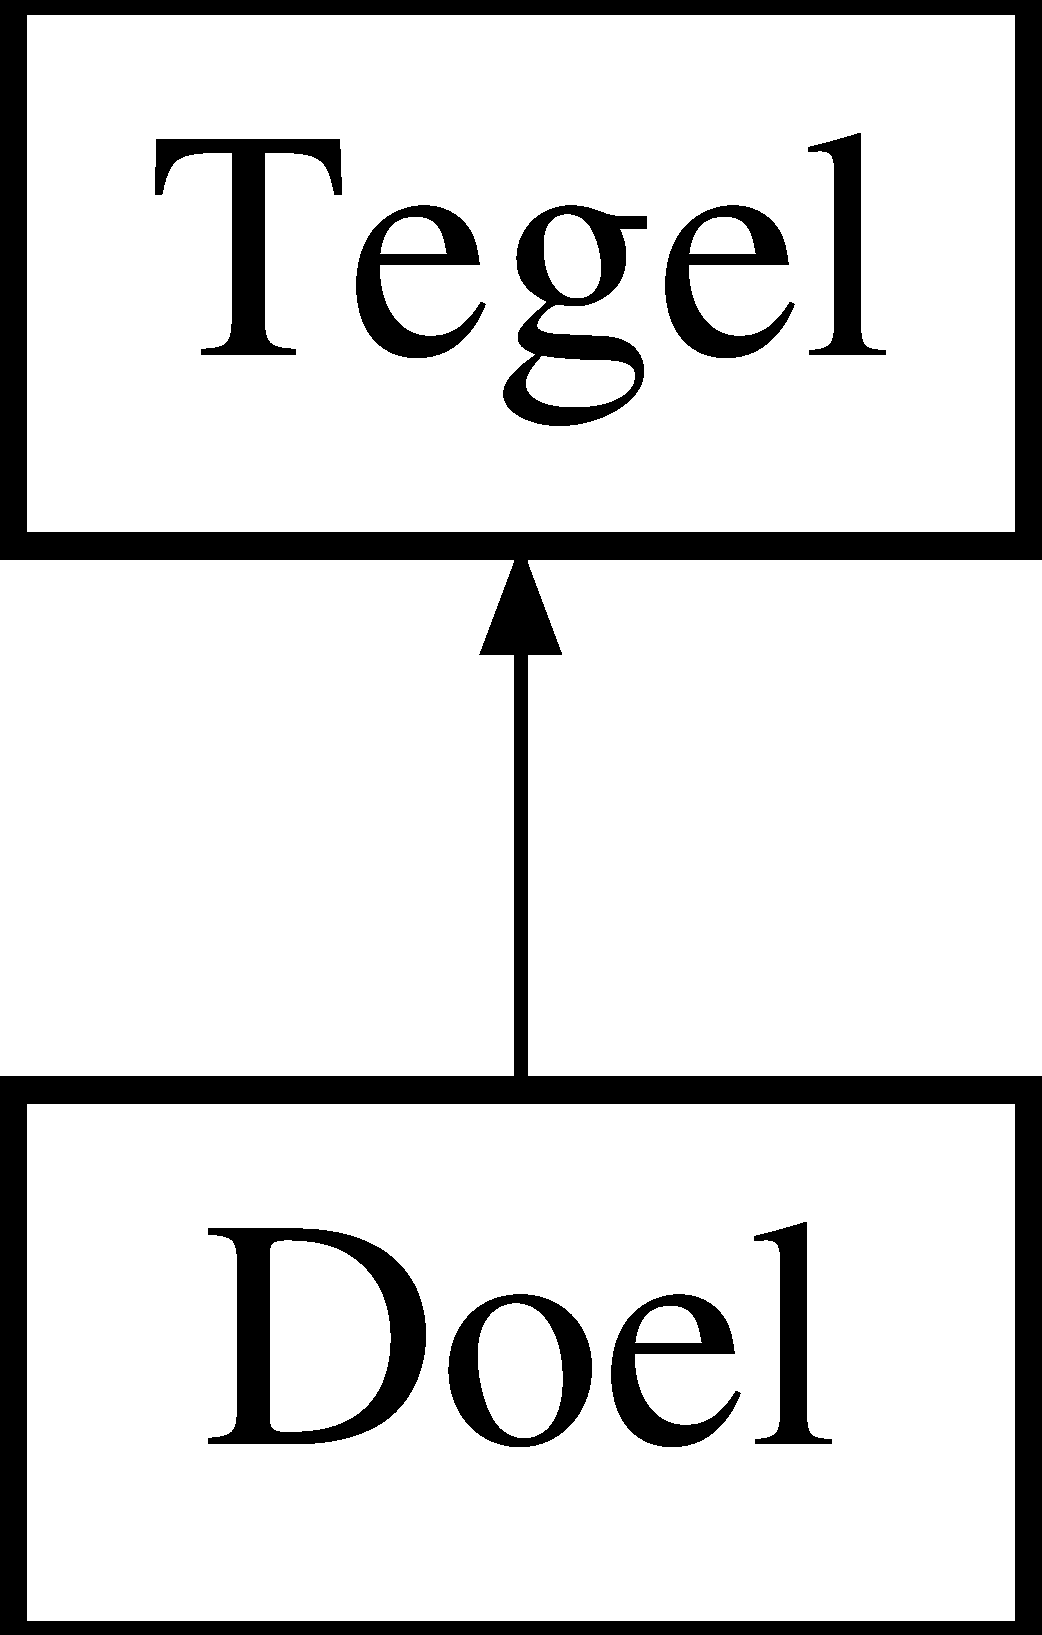
\includegraphics[height=2.000000cm]{class_doel}
\end{center}
\end{figure}
\subsection*{Public Member Functions}
\begin{DoxyCompactItemize}
\item 
\hyperlink{class_doel_a0a40326f08f54e04c19539eb36078b1a}{Doel} (int x, int y)
\item 
int \hyperlink{class_doel_aa12ca3c1dd4f7855c77d36f959bdf52c}{get\+Positie} ()
\item 
void \hyperlink{class_doel_aeaf533cd25c7b2d21a0d3d6f20469415}{update} (\hyperlink{classkey_manager}{key\+Manager} \hyperlink{classkey_manager}{key\+Manager})
\item 
void \hyperlink{class_doel_a8c88c577bc902337fb8b4803fc8a90b7}{render} (Graphics g, Buffer\+Strategy bs)
\end{DoxyCompactItemize}
\subsection*{Additional Inherited Members}


\subsection{Detailed Description}
\begin{DoxyAuthor}{Author}
Kelvin 

Senne 

Corn� 

Jordy 

Aran
\end{DoxyAuthor}
\begin{DoxyVersion}{Version}
1.\+1 03/6/2017 
\end{DoxyVersion}
\begin{DoxySince}{Since}
1.\+0
\end{DoxySince}
This class makes the goal 

\subsection{Constructor \& Destructor Documentation}
\mbox{\Hypertarget{class_doel_a0a40326f08f54e04c19539eb36078b1a}\label{class_doel_a0a40326f08f54e04c19539eb36078b1a}} 
\index{Doel@{Doel}!Doel@{Doel}}
\index{Doel@{Doel}!Doel@{Doel}}
\subsubsection{\texorpdfstring{Doel()}{Doel()}}
{\footnotesize\ttfamily Doel.\+Doel (\begin{DoxyParamCaption}\item[{int}]{x,  }\item[{int}]{y }\end{DoxyParamCaption})}

Constructor takes the x and y, and give this to \hyperlink{class_tegel}{Tegel} constructor with \char`\"{}super()\char`\"{} 
\begin{DoxyParams}{Parameters}
{\em x} & ; Used for the horizontal position \\
\hline
{\em y} & ; Used for the vertical position \\
\hline
\end{DoxyParams}
\begin{DoxySeeAlso}{See also}
\hyperlink{class_tegel}{Tegel} Constructor 
\end{DoxySeeAlso}


\subsection{Member Function Documentation}
\mbox{\Hypertarget{class_doel_aa12ca3c1dd4f7855c77d36f959bdf52c}\label{class_doel_aa12ca3c1dd4f7855c77d36f959bdf52c}} 
\index{Doel@{Doel}!get\+Positie@{get\+Positie}}
\index{get\+Positie@{get\+Positie}!Doel@{Doel}}
\subsubsection{\texorpdfstring{get\+Positie()}{getPositie()}}
{\footnotesize\ttfamily int Doel.\+get\+Positie (\begin{DoxyParamCaption}{ }\end{DoxyParamCaption})}

This method does nothing \mbox{\Hypertarget{class_doel_a8c88c577bc902337fb8b4803fc8a90b7}\label{class_doel_a8c88c577bc902337fb8b4803fc8a90b7}} 
\index{Doel@{Doel}!render@{render}}
\index{render@{render}!Doel@{Doel}}
\subsubsection{\texorpdfstring{render()}{render()}}
{\footnotesize\ttfamily void Doel.\+render (\begin{DoxyParamCaption}\item[{Graphics}]{g,  }\item[{Buffer\+Strategy}]{bs }\end{DoxyParamCaption})}

This method does nothing \mbox{\Hypertarget{class_doel_aeaf533cd25c7b2d21a0d3d6f20469415}\label{class_doel_aeaf533cd25c7b2d21a0d3d6f20469415}} 
\index{Doel@{Doel}!update@{update}}
\index{update@{update}!Doel@{Doel}}
\subsubsection{\texorpdfstring{update()}{update()}}
{\footnotesize\ttfamily void Doel.\+update (\begin{DoxyParamCaption}\item[{\hyperlink{classkey_manager}{key\+Manager}}]{key\+Manager }\end{DoxyParamCaption})}

This method does nothing 

The documentation for this class was generated from the following file\+:\begin{DoxyCompactItemize}
\item 
D\+:/users/senne/workspace/\+No\+Game/src/Doel.\+java\end{DoxyCompactItemize}

\hypertarget{classimage_loader}{}\section{image\+Loader Class Reference}
\label{classimage_loader}\index{image\+Loader@{image\+Loader}}
\subsection*{Static Public Member Functions}
\begin{DoxyCompactItemize}
\item 
\mbox{\Hypertarget{classimage_loader_ac30615d1b0e62305fe44d6070ea32a43}\label{classimage_loader_ac30615d1b0e62305fe44d6070ea32a43}} 
static Buffered\+Image {\bfseries load\+Image} (String path)
\end{DoxyCompactItemize}


\subsection{Detailed Description}
\begin{DoxyAuthor}{Author}
Kelvin 

Senne 

Corn� 

Jordy 

Aran
\end{DoxyAuthor}
\begin{DoxyVersion}{Version}
1.\+1 03/6/2017 
\end{DoxyVersion}
\begin{DoxySince}{Since}
1.\+1
\end{DoxySince}
This class is used for Buffer\+Image\+Strategy 

The documentation for this class was generated from the following file\+:\begin{DoxyCompactItemize}
\item 
D\+:/users/senne/workspace/\+No\+Game/src/image\+Loader.\+java\end{DoxyCompactItemize}

\hypertarget{classkey_manager}{}\section{key\+Manager Class Reference}
\label{classkey_manager}\index{key\+Manager@{key\+Manager}}
Inheritance diagram for key\+Manager\+:\begin{figure}[H]
\begin{center}
\leavevmode
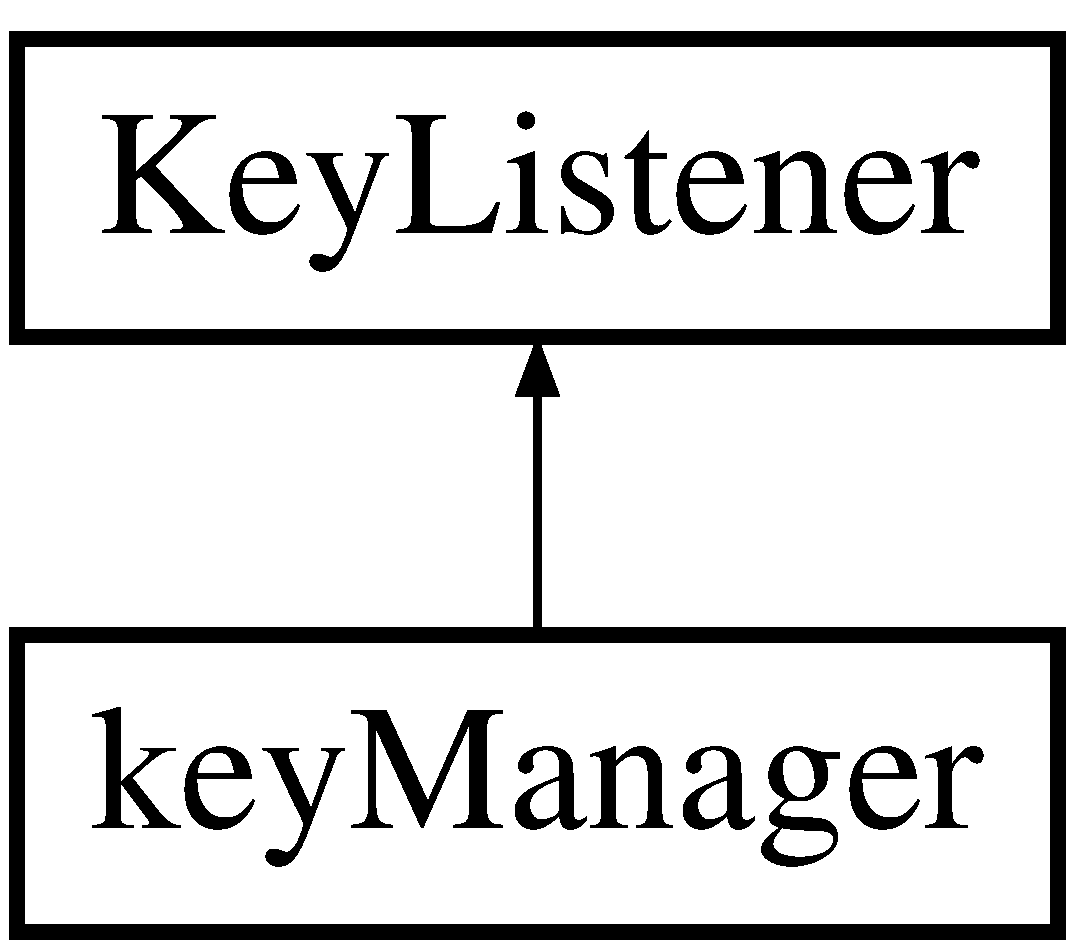
\includegraphics[height=2.000000cm]{classkey_manager}
\end{center}
\end{figure}
\subsection*{Public Member Functions}
\begin{DoxyCompactItemize}
\item 
\hyperlink{classkey_manager_a0b560329b1fe90f14bf962293f08d48b}{key\+Manager} ()
\item 
void \hyperlink{classkey_manager_aeca54bd359289741b30016274729ad4e}{update} ()
\item 
void \hyperlink{classkey_manager_a025dad8f0eec442c8cd19cd20c3635c7}{key\+Pressed} (Key\+Event e)
\item 
void \hyperlink{classkey_manager_a7635b0f0d8e3266c35b33f4e44bd6e42}{key\+Released} (Key\+Event e)
\item 
void \hyperlink{classkey_manager_a1f4f493c92e64239b6d23139de91babf}{key\+Typed} (Key\+Event e)
\end{DoxyCompactItemize}
\subsection*{Public Attributes}
\begin{DoxyCompactItemize}
\item 
\mbox{\Hypertarget{classkey_manager_a43aadbfe02926e78a4fcea96152ed21a}\label{classkey_manager_a43aadbfe02926e78a4fcea96152ed21a}} 
boolean {\bfseries up}
\item 
\mbox{\Hypertarget{classkey_manager_aae955a49a4891073fe0a9afb6ad6c658}\label{classkey_manager_aae955a49a4891073fe0a9afb6ad6c658}} 
boolean {\bfseries kan\+Indrukken} = true
\end{DoxyCompactItemize}


\subsection{Detailed Description}
This class makes the goal \begin{DoxyAuthor}{Author}
Kelvin 

Senne 

Corn� 

Jordy 

Aran
\end{DoxyAuthor}
\begin{DoxyVersion}{Version}
1.\+1 03/6/2017 
\end{DoxyVersion}
\begin{DoxySince}{Since}
1.\+1
\end{DoxySince}
This class is used to move

Used sources\+: 
\begin{DoxyItemize}
\item \href{http://stackoverflow.com/questions/2623995/swings-keylistener-and-multiple-keys-pressed-at-the-same-time}{\tt http\+://stackoverflow.\+com/questions/2623995/swings-\/keylistener-\/and-\/multiple-\/keys-\/pressed-\/at-\/the-\/same-\/time} 
\end{DoxyItemize}

\subsection{Constructor \& Destructor Documentation}
\mbox{\Hypertarget{classkey_manager_a0b560329b1fe90f14bf962293f08d48b}\label{classkey_manager_a0b560329b1fe90f14bf962293f08d48b}} 
\index{key\+Manager@{key\+Manager}!key\+Manager@{key\+Manager}}
\index{key\+Manager@{key\+Manager}!key\+Manager@{key\+Manager}}
\subsubsection{\texorpdfstring{key\+Manager()}{keyManager()}}
{\footnotesize\ttfamily key\+Manager.\+key\+Manager (\begin{DoxyParamCaption}{ }\end{DoxyParamCaption})}

Constructor uses the keys array to fill it with booleans. 

\subsection{Member Function Documentation}
\mbox{\Hypertarget{classkey_manager_a025dad8f0eec442c8cd19cd20c3635c7}\label{classkey_manager_a025dad8f0eec442c8cd19cd20c3635c7}} 
\index{key\+Manager@{key\+Manager}!key\+Pressed@{key\+Pressed}}
\index{key\+Pressed@{key\+Pressed}!key\+Manager@{key\+Manager}}
\subsubsection{\texorpdfstring{key\+Pressed()}{keyPressed()}}
{\footnotesize\ttfamily void key\+Manager.\+key\+Pressed (\begin{DoxyParamCaption}\item[{Key\+Event}]{e }\end{DoxyParamCaption})}

If a key is pressed this method is called, When a key is already pressed, no other can be used. \mbox{\Hypertarget{classkey_manager_a7635b0f0d8e3266c35b33f4e44bd6e42}\label{classkey_manager_a7635b0f0d8e3266c35b33f4e44bd6e42}} 
\index{key\+Manager@{key\+Manager}!key\+Released@{key\+Released}}
\index{key\+Released@{key\+Released}!key\+Manager@{key\+Manager}}
\subsubsection{\texorpdfstring{key\+Released()}{keyReleased()}}
{\footnotesize\ttfamily void key\+Manager.\+key\+Released (\begin{DoxyParamCaption}\item[{Key\+Event}]{e }\end{DoxyParamCaption})}

If a key is released this method is called, So a new key can be pressed. \mbox{\Hypertarget{classkey_manager_a1f4f493c92e64239b6d23139de91babf}\label{classkey_manager_a1f4f493c92e64239b6d23139de91babf}} 
\index{key\+Manager@{key\+Manager}!key\+Typed@{key\+Typed}}
\index{key\+Typed@{key\+Typed}!key\+Manager@{key\+Manager}}
\subsubsection{\texorpdfstring{key\+Typed()}{keyTyped()}}
{\footnotesize\ttfamily void key\+Manager.\+key\+Typed (\begin{DoxyParamCaption}\item[{Key\+Event}]{e }\end{DoxyParamCaption})}

This method is not used \mbox{\Hypertarget{classkey_manager_aeca54bd359289741b30016274729ad4e}\label{classkey_manager_aeca54bd359289741b30016274729ad4e}} 
\index{key\+Manager@{key\+Manager}!update@{update}}
\index{update@{update}!key\+Manager@{key\+Manager}}
\subsubsection{\texorpdfstring{update()}{update()}}
{\footnotesize\ttfamily void key\+Manager.\+update (\begin{DoxyParamCaption}{ }\end{DoxyParamCaption})}

This method is used to update the keys W, S, A, D 

The documentation for this class was generated from the following file\+:\begin{DoxyCompactItemize}
\item 
D\+:/users/senne/workspace/\+No\+Game/src/key\+Manager.\+java\end{DoxyCompactItemize}

\hypertarget{class_leeg}{}\section{Leeg Class Reference}
\label{class_leeg}\index{Leeg@{Leeg}}
Inheritance diagram for Leeg\+:\begin{figure}[H]
\begin{center}
\leavevmode
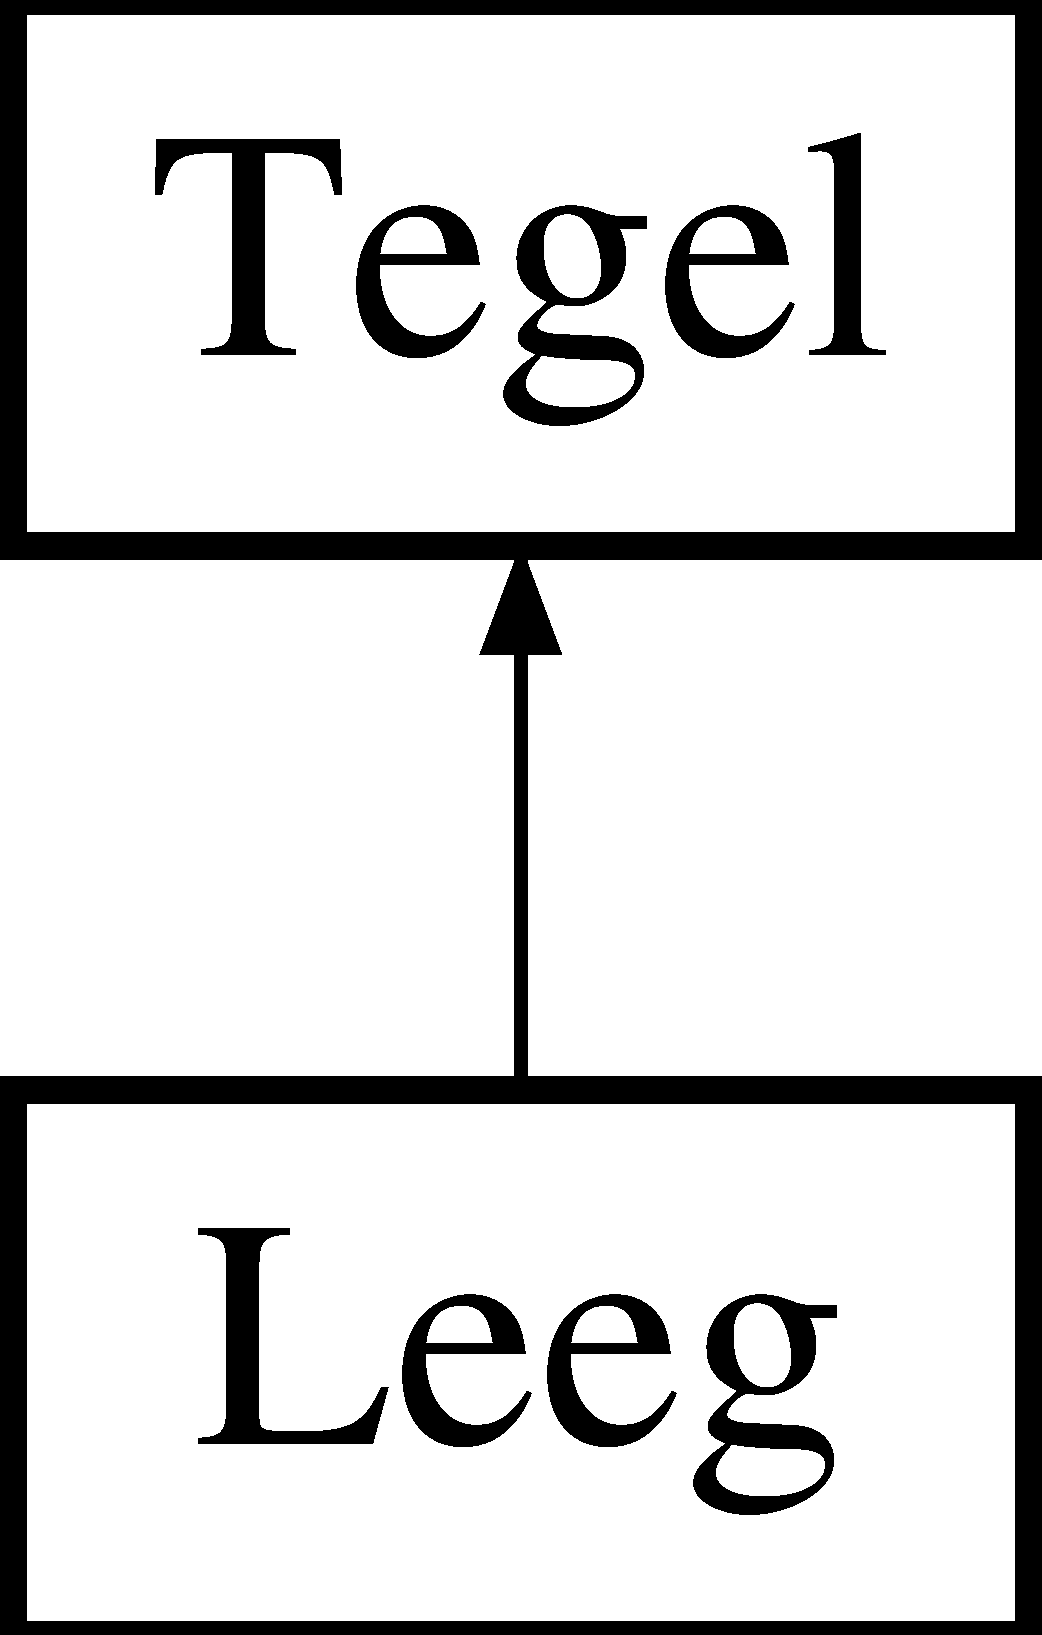
\includegraphics[height=2.000000cm]{class_leeg}
\end{center}
\end{figure}
\subsection*{Public Member Functions}
\begin{DoxyCompactItemize}
\item 
\hyperlink{class_leeg_a050cdd15d9b300162c69bcbccb008618}{Leeg} (int x, int y)
\item 
int \hyperlink{class_leeg_ace54d83ab69cb1b34652caeec793c70a}{get\+Positie} ()
\item 
void \hyperlink{class_leeg_a9290f0bb08ec4faabb9836c041281c01}{update} (\hyperlink{classkey_manager}{key\+Manager} \hyperlink{classkey_manager}{key\+Manager})
\item 
void \hyperlink{class_leeg_aa22049cbaeb3f2b36b484aadf5dd6058}{render} (Graphics g, Buffer\+Strategy bs)
\end{DoxyCompactItemize}
\subsection*{Additional Inherited Members}


\subsection{Detailed Description}
\begin{DoxyAuthor}{Author}
Kelvin 

Senne 

Corn� 

Jordy 

Aran
\end{DoxyAuthor}
\begin{DoxyVersion}{Version}
1.\+1 03/6/2017 
\end{DoxyVersion}
\begin{DoxySince}{Since}
1.\+0
\end{DoxySince}
This class creates the empty tile 

\subsection{Constructor \& Destructor Documentation}
\mbox{\Hypertarget{class_leeg_a050cdd15d9b300162c69bcbccb008618}\label{class_leeg_a050cdd15d9b300162c69bcbccb008618}} 
\index{Leeg@{Leeg}!Leeg@{Leeg}}
\index{Leeg@{Leeg}!Leeg@{Leeg}}
\subsubsection{\texorpdfstring{Leeg()}{Leeg()}}
{\footnotesize\ttfamily Leeg.\+Leeg (\begin{DoxyParamCaption}\item[{int}]{x,  }\item[{int}]{y }\end{DoxyParamCaption})}

Constructor takes the x and y, and give this to \hyperlink{class_tegel}{Tegel} constructor with \char`\"{}super()\char`\"{} 
\begin{DoxyParams}{Parameters}
{\em x} & ; Used for the horizontal position \\
\hline
{\em y} & ; Used for the vertical position \\
\hline
\end{DoxyParams}
\begin{DoxySeeAlso}{See also}
\hyperlink{class_tegel}{Tegel} Constructor 
\end{DoxySeeAlso}


\subsection{Member Function Documentation}
\mbox{\Hypertarget{class_leeg_ace54d83ab69cb1b34652caeec793c70a}\label{class_leeg_ace54d83ab69cb1b34652caeec793c70a}} 
\index{Leeg@{Leeg}!get\+Positie@{get\+Positie}}
\index{get\+Positie@{get\+Positie}!Leeg@{Leeg}}
\subsubsection{\texorpdfstring{get\+Positie()}{getPositie()}}
{\footnotesize\ttfamily int Leeg.\+get\+Positie (\begin{DoxyParamCaption}{ }\end{DoxyParamCaption})}

This method does nothing \mbox{\Hypertarget{class_leeg_aa22049cbaeb3f2b36b484aadf5dd6058}\label{class_leeg_aa22049cbaeb3f2b36b484aadf5dd6058}} 
\index{Leeg@{Leeg}!render@{render}}
\index{render@{render}!Leeg@{Leeg}}
\subsubsection{\texorpdfstring{render()}{render()}}
{\footnotesize\ttfamily void Leeg.\+render (\begin{DoxyParamCaption}\item[{Graphics}]{g,  }\item[{Buffer\+Strategy}]{bs }\end{DoxyParamCaption})}

This method does nothing \mbox{\Hypertarget{class_leeg_a9290f0bb08ec4faabb9836c041281c01}\label{class_leeg_a9290f0bb08ec4faabb9836c041281c01}} 
\index{Leeg@{Leeg}!update@{update}}
\index{update@{update}!Leeg@{Leeg}}
\subsubsection{\texorpdfstring{update()}{update()}}
{\footnotesize\ttfamily void Leeg.\+update (\begin{DoxyParamCaption}\item[{\hyperlink{classkey_manager}{key\+Manager}}]{key\+Manager }\end{DoxyParamCaption})}

This method does nothing 

The documentation for this class was generated from the following file\+:\begin{DoxyCompactItemize}
\item 
D\+:/users/senne/workspace/\+No\+Game/src/Leeg.\+java\end{DoxyCompactItemize}

\hypertarget{class_locatie}{}\section{Locatie Class Reference}
\label{class_locatie}\index{Locatie@{Locatie}}
\subsection*{Public Member Functions}
\begin{DoxyCompactItemize}
\item 
\hyperlink{class_locatie_a75039c470f59d768b6e29a5ac98fffbb}{Locatie} (int x, int y)
\item 
int \hyperlink{class_locatie_af5745c91737bb28043d88475021f311c}{getX} ()
\item 
int \hyperlink{class_locatie_a884b44635de0c575afcfe9f102966578}{getY} ()
\item 
void \hyperlink{class_locatie_a46e75e465c8584b10746739bcab9e5f1}{set\+XY} (\hyperlink{enum_richting}{Richting} richting)
\end{DoxyCompactItemize}


\subsection{Detailed Description}
This class makes the goal \begin{DoxyAuthor}{Author}
Kelvin 

Senne 

Corn� 

Jordy 

Aran
\end{DoxyAuthor}
\begin{DoxyVersion}{Version}
1.\+1 03/6/2017 
\end{DoxyVersion}
\begin{DoxySince}{Since}
1.\+1
\end{DoxySince}
This class is used to store the location of a tile. And set it or give it back 

\subsection{Constructor \& Destructor Documentation}
\mbox{\Hypertarget{class_locatie_a75039c470f59d768b6e29a5ac98fffbb}\label{class_locatie_a75039c470f59d768b6e29a5ac98fffbb}} 
\index{Locatie@{Locatie}!Locatie@{Locatie}}
\index{Locatie@{Locatie}!Locatie@{Locatie}}
\subsubsection{\texorpdfstring{Locatie()}{Locatie()}}
{\footnotesize\ttfamily Locatie.\+Locatie (\begin{DoxyParamCaption}\item[{int}]{x,  }\item[{int}]{y }\end{DoxyParamCaption})}


\begin{DoxyParams}{Parameters}
{\em x} & ; Used for the horizontal position \\
\hline
{\em y} & ; Used for the vertical position \\
\hline
\end{DoxyParams}


\subsection{Member Function Documentation}
\mbox{\Hypertarget{class_locatie_af5745c91737bb28043d88475021f311c}\label{class_locatie_af5745c91737bb28043d88475021f311c}} 
\index{Locatie@{Locatie}!getX@{getX}}
\index{getX@{getX}!Locatie@{Locatie}}
\subsubsection{\texorpdfstring{get\+X()}{getX()}}
{\footnotesize\ttfamily int Locatie.\+getX (\begin{DoxyParamCaption}{ }\end{DoxyParamCaption})}

\begin{DoxyReturn}{Returns}
x ; it is multiplied by 50 to represent the pixels 
\end{DoxyReturn}
\mbox{\Hypertarget{class_locatie_a884b44635de0c575afcfe9f102966578}\label{class_locatie_a884b44635de0c575afcfe9f102966578}} 
\index{Locatie@{Locatie}!getY@{getY}}
\index{getY@{getY}!Locatie@{Locatie}}
\subsubsection{\texorpdfstring{get\+Y()}{getY()}}
{\footnotesize\ttfamily int Locatie.\+getY (\begin{DoxyParamCaption}{ }\end{DoxyParamCaption})}

\begin{DoxyReturn}{Returns}
y ; it is multiplied by 50 to represent the pixels 
\end{DoxyReturn}
\mbox{\Hypertarget{class_locatie_a46e75e465c8584b10746739bcab9e5f1}\label{class_locatie_a46e75e465c8584b10746739bcab9e5f1}} 
\index{Locatie@{Locatie}!set\+XY@{set\+XY}}
\index{set\+XY@{set\+XY}!Locatie@{Locatie}}
\subsubsection{\texorpdfstring{set\+X\+Y()}{setXY()}}
{\footnotesize\ttfamily void Locatie.\+set\+XY (\begin{DoxyParamCaption}\item[{\hyperlink{enum_richting}{Richting}}]{richting }\end{DoxyParamCaption})}

This method is used to set the x and y coordinates 
\begin{DoxyParams}{Parameters}
{\em x} & ; Used for the horizontal position \\
\hline
{\em y} & ; Used for the vertical position \\
\hline
\end{DoxyParams}


The documentation for this class was generated from the following file\+:\begin{DoxyCompactItemize}
\item 
D\+:/users/senne/workspace/\+No\+Game/src/Locatie.\+java\end{DoxyCompactItemize}

\hypertarget{class_main_frame}{}\section{Main\+Frame Class Reference}
\label{class_main_frame}\index{Main\+Frame@{Main\+Frame}}
\subsection*{Static Public Member Functions}
\begin{DoxyCompactItemize}
\item 
\mbox{\Hypertarget{class_main_frame_aa24e10bb8d7e55f4bd1cba7722167e84}\label{class_main_frame_aa24e10bb8d7e55f4bd1cba7722167e84}} 
static void {\bfseries main} (String\mbox{[}$\,$\mbox{]} args)
\end{DoxyCompactItemize}


\subsection{Detailed Description}
This class makes the goal \begin{DoxyAuthor}{Author}
Kelvin 

Senne 

Corn� 

Jordy 

Aran
\end{DoxyAuthor}
\begin{DoxyVersion}{Version}
1.\+1 03/6/2017 
\end{DoxyVersion}
\begin{DoxySince}{Since}
1.\+0
\end{DoxySince}
This class is the main which is used for starting the game

Used sources\+: 
\begin{DoxyItemize}
\item \href{http://docs.oracle.com/javase/tutorial/uiswing/painting/step1.html}{\tt http\+://docs.\+oracle.\+com/javase/tutorial/uiswing/painting/step1.\+html} 
\item \href{https://github.com/CodeNMore/New-Beginner-Java-Game-Programming-Src/blob/master/Episode%204/TileGame/src/dev/codenmore/tilegame/Game.java}{\tt https\+://github.\+com/\+Code\+N\+More/\+New-\/\+Beginner-\/\+Java-\/\+Game-\/\+Programming-\/\+Src/blob/master/\+Episode\%204/\+Tile\+Game/src/dev/codenmore/tilegame/\+Game.\+java} 
\end{DoxyItemize}

The documentation for this class was generated from the following file\+:\begin{DoxyCompactItemize}
\item 
D\+:/users/senne/workspace/\+No\+Game/src/Main\+Frame.\+java\end{DoxyCompactItemize}

\hypertarget{class_muur}{}\section{Muur Class Reference}
\label{class_muur}\index{Muur@{Muur}}
Inheritance diagram for Muur\+:\begin{figure}[H]
\begin{center}
\leavevmode
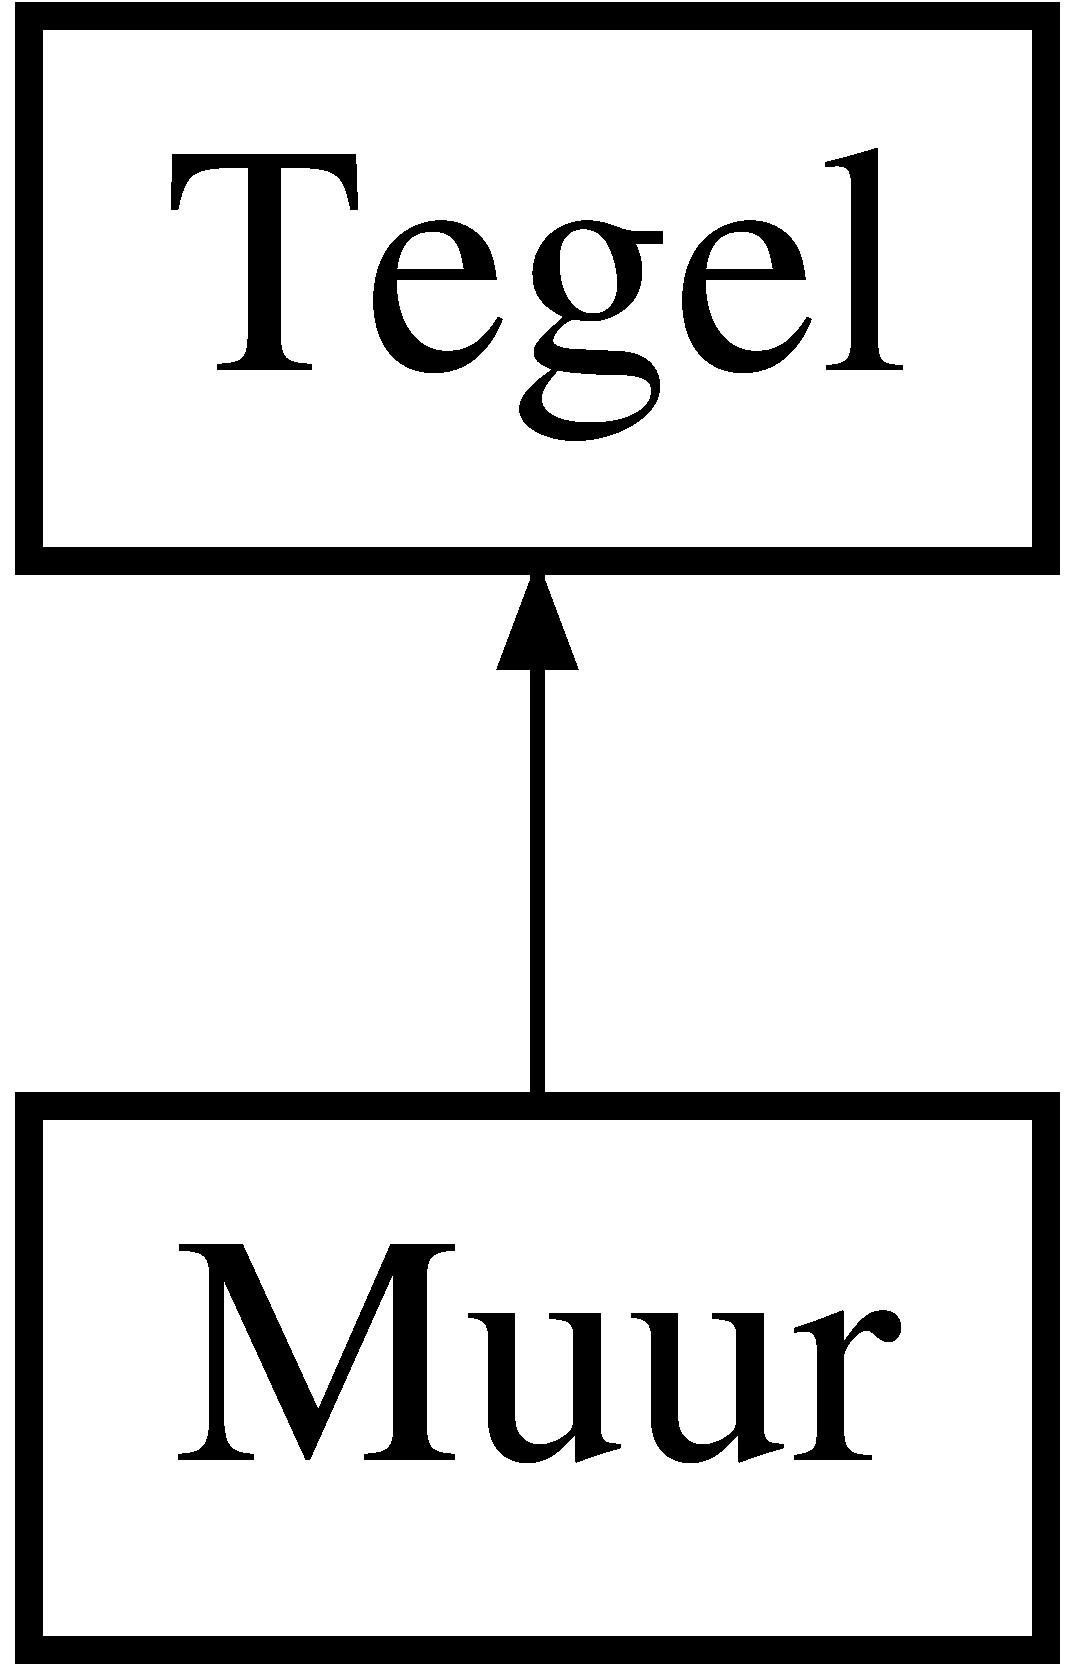
\includegraphics[height=2.000000cm]{class_muur}
\end{center}
\end{figure}
\subsection*{Public Member Functions}
\begin{DoxyCompactItemize}
\item 
\hyperlink{class_muur_a8ffdee68307e226f38a2939af941fd22}{Muur} (int x, int y)
\item 
int \hyperlink{class_muur_a053be14281cc198795019ec6fdbe0cf3}{get\+Positie} ()
\item 
void \hyperlink{class_muur_a514aee7304a3d2c71e8ac969b7a3512b}{update} (\hyperlink{classkey_manager}{key\+Manager} \hyperlink{classkey_manager}{key\+Manager})
\item 
void \hyperlink{class_muur_a4b02b5e679b752ca9762115977fbe8c0}{render} (Graphics g, Buffer\+Strategy bs)
\end{DoxyCompactItemize}
\subsection*{Additional Inherited Members}


\subsection{Detailed Description}
\begin{DoxyAuthor}{Author}
Kelvin 

Senne 

Corn� 

Jordy 

Aran
\end{DoxyAuthor}
\begin{DoxyVersion}{Version}
1.\+1 03/6/2017 
\end{DoxyVersion}
\begin{DoxySince}{Since}
1.\+0
\end{DoxySince}
This class creates the empty tile 

\subsection{Constructor \& Destructor Documentation}
\mbox{\Hypertarget{class_muur_a8ffdee68307e226f38a2939af941fd22}\label{class_muur_a8ffdee68307e226f38a2939af941fd22}} 
\index{Muur@{Muur}!Muur@{Muur}}
\index{Muur@{Muur}!Muur@{Muur}}
\subsubsection{\texorpdfstring{Muur()}{Muur()}}
{\footnotesize\ttfamily Muur.\+Muur (\begin{DoxyParamCaption}\item[{int}]{x,  }\item[{int}]{y }\end{DoxyParamCaption})}

Constructor takes the x and y, and give this to \hyperlink{class_tegel}{Tegel} constructor with \char`\"{}super()\char`\"{} 
\begin{DoxyParams}{Parameters}
{\em x} & ; Used for the horizontal position \\
\hline
{\em y} & ; Used for the vertical position \\
\hline
\end{DoxyParams}
\begin{DoxySeeAlso}{See also}
\hyperlink{class_tegel}{Tegel} Constructor 
\end{DoxySeeAlso}


\subsection{Member Function Documentation}
\mbox{\Hypertarget{class_muur_a053be14281cc198795019ec6fdbe0cf3}\label{class_muur_a053be14281cc198795019ec6fdbe0cf3}} 
\index{Muur@{Muur}!get\+Positie@{get\+Positie}}
\index{get\+Positie@{get\+Positie}!Muur@{Muur}}
\subsubsection{\texorpdfstring{get\+Positie()}{getPositie()}}
{\footnotesize\ttfamily int Muur.\+get\+Positie (\begin{DoxyParamCaption}{ }\end{DoxyParamCaption})}

This method does nothing \mbox{\Hypertarget{class_muur_a4b02b5e679b752ca9762115977fbe8c0}\label{class_muur_a4b02b5e679b752ca9762115977fbe8c0}} 
\index{Muur@{Muur}!render@{render}}
\index{render@{render}!Muur@{Muur}}
\subsubsection{\texorpdfstring{render()}{render()}}
{\footnotesize\ttfamily void Muur.\+render (\begin{DoxyParamCaption}\item[{Graphics}]{g,  }\item[{Buffer\+Strategy}]{bs }\end{DoxyParamCaption})}

This method does nothing \mbox{\Hypertarget{class_muur_a514aee7304a3d2c71e8ac969b7a3512b}\label{class_muur_a514aee7304a3d2c71e8ac969b7a3512b}} 
\index{Muur@{Muur}!update@{update}}
\index{update@{update}!Muur@{Muur}}
\subsubsection{\texorpdfstring{update()}{update()}}
{\footnotesize\ttfamily void Muur.\+update (\begin{DoxyParamCaption}\item[{\hyperlink{classkey_manager}{key\+Manager}}]{key\+Manager }\end{DoxyParamCaption})}

This method does nothing 

The documentation for this class was generated from the following file\+:\begin{DoxyCompactItemize}
\item 
D\+:/users/senne/workspace/\+No\+Game/src/Muur.\+java\end{DoxyCompactItemize}

\hypertarget{enum_richting}{}\section{Richting Enum Reference}
\label{enum_richting}\index{Richting@{Richting}}
\subsection*{Public Member Functions}
\begin{DoxyCompactItemize}
\item 
int \hyperlink{enum_richting_a58a10e4858f6b3389b525e8a9e32ba11}{getX} ()
\item 
int \hyperlink{enum_richting_a8b345f9df8953bf86da892faaa73927e}{getY} ()
\end{DoxyCompactItemize}
\subsection*{Public Attributes}
\begin{DoxyCompactItemize}
\item 
\mbox{\Hypertarget{enum_richting_a8ba9b60b36cad0fe3b56c43b5c9e852f}\label{enum_richting_a8ba9b60b36cad0fe3b56c43b5c9e852f}} 
{\bfseries N\+O\+O\+RD} =(0, -\/1)
\item 
\mbox{\Hypertarget{enum_richting_a295abb737aad694227e7eae3cb750cea}\label{enum_richting_a295abb737aad694227e7eae3cb750cea}} 
{\bfseries O\+O\+ST} =(1, 0)
\item 
\mbox{\Hypertarget{enum_richting_aa47d6eae94fe816441caaf6b347aa55f}\label{enum_richting_aa47d6eae94fe816441caaf6b347aa55f}} 
{\bfseries Z\+U\+ID} =(0, 1)
\item 
\mbox{\Hypertarget{enum_richting_a0b35767f6d26983dd50fe9b5c0715d37}\label{enum_richting_a0b35767f6d26983dd50fe9b5c0715d37}} 
{\bfseries W\+E\+ST} =(-\/1,0)
\item 
\mbox{\Hypertarget{enum_richting_ab7d663bec066d8be163c6125a9631110}\label{enum_richting_ab7d663bec066d8be163c6125a9631110}} 
int {\bfseries dk}
\end{DoxyCompactItemize}


\subsection{Detailed Description}
\begin{DoxyAuthor}{Author}
Kelvin 

Senne 

Corn� 

Jordy 

Aran 
\end{DoxyAuthor}
\begin{DoxyVersion}{Version}
1.\+1 03/6/2017 
\end{DoxyVersion}
\begin{DoxySince}{Since}
1.\+1
\end{DoxySince}
Enum gives the direction N\+O\+R\+TH, E\+A\+ST, W\+E\+ST and S\+O\+U\+TH 

\subsection{Member Function Documentation}
\mbox{\Hypertarget{enum_richting_a58a10e4858f6b3389b525e8a9e32ba11}\label{enum_richting_a58a10e4858f6b3389b525e8a9e32ba11}} 
\index{Richting@{Richting}!getX@{getX}}
\index{getX@{getX}!Richting@{Richting}}
\subsubsection{\texorpdfstring{get\+X()}{getX()}}
{\footnotesize\ttfamily int Richting.\+getX (\begin{DoxyParamCaption}{ }\end{DoxyParamCaption})}

\begin{DoxyReturn}{Returns}
dr ; aka X 
\end{DoxyReturn}
\mbox{\Hypertarget{enum_richting_a8b345f9df8953bf86da892faaa73927e}\label{enum_richting_a8b345f9df8953bf86da892faaa73927e}} 
\index{Richting@{Richting}!getY@{getY}}
\index{getY@{getY}!Richting@{Richting}}
\subsubsection{\texorpdfstring{get\+Y()}{getY()}}
{\footnotesize\ttfamily int Richting.\+getY (\begin{DoxyParamCaption}{ }\end{DoxyParamCaption})}

\begin{DoxyReturn}{Returns}
dk ; aka Y 
\end{DoxyReturn}


The documentation for this enum was generated from the following file\+:\begin{DoxyCompactItemize}
\item 
D\+:/users/senne/workspace/\+No\+Game/src/Richting.\+java\end{DoxyCompactItemize}

\hypertarget{class_speelveld}{}\section{Speelveld Class Reference}
\label{class_speelveld}\index{Speelveld@{Speelveld}}
Inheritance diagram for Speelveld\+:\begin{figure}[H]
\begin{center}
\leavevmode
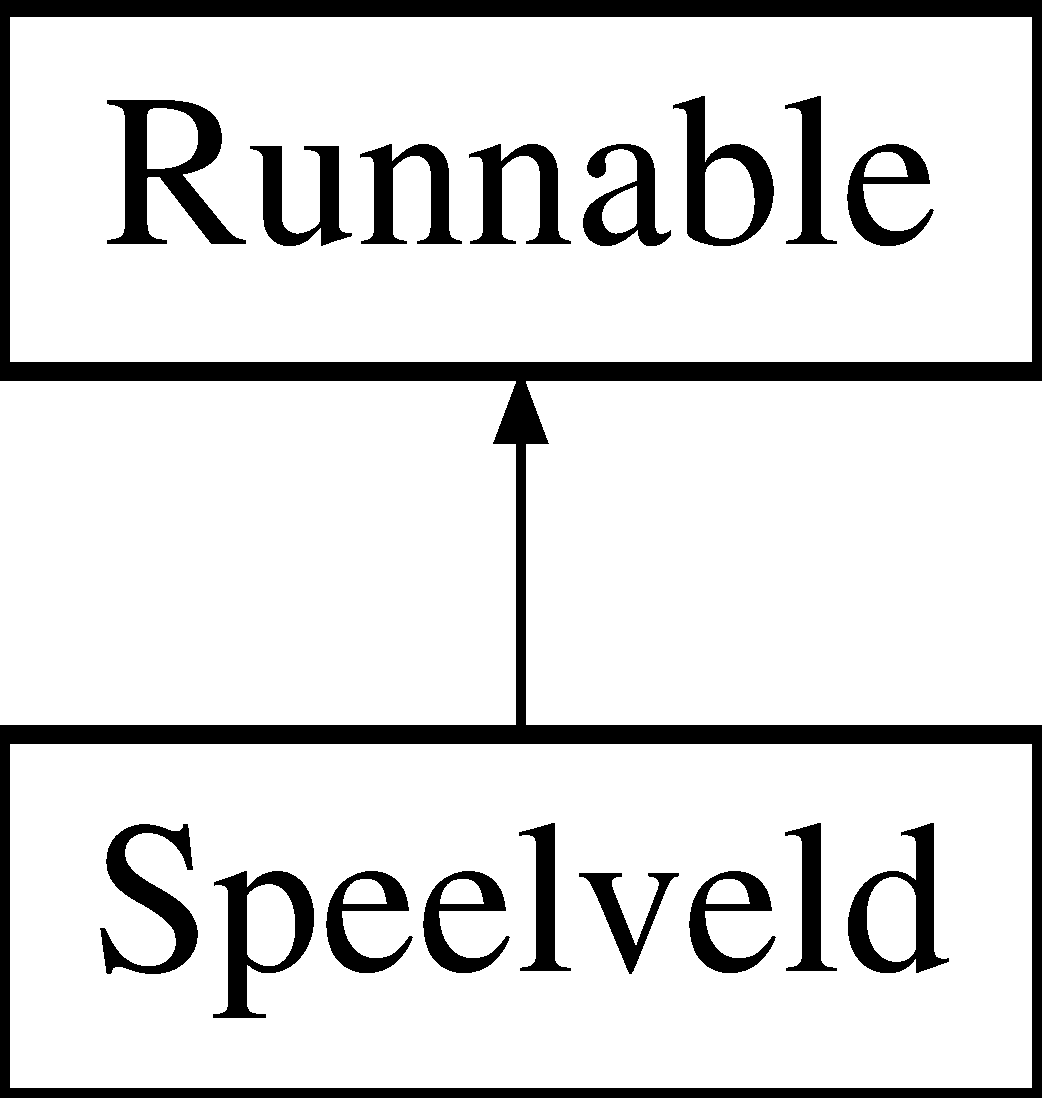
\includegraphics[height=2.000000cm]{class_speelveld}
\end{center}
\end{figure}
\subsection*{Public Member Functions}
\begin{DoxyCompactItemize}
\item 
\hyperlink{class_speelveld_a3b0312c68b60dd3e9fc5e2409e9ccc17}{Speelveld} (int aantal\+Rijen, int aantal\+Kolommen, int level)
\item 
void \hyperlink{class_speelveld_a654b50c9419077aeafba7be2e3d310c3}{run} ()
\item 
synchronized void \hyperlink{class_speelveld_afdcb7b7519b450cfc2bdf767363dc685}{start} ()
\item 
synchronized void \hyperlink{class_speelveld_aeb175779ea45a292beb6e25752daeec6}{stop} ()
\end{DoxyCompactItemize}


\subsection{Detailed Description}
\begin{DoxyAuthor}{Author}
Kelvin 

Senne 

Corn� 

Jordy 

Aran 
\end{DoxyAuthor}
\begin{DoxyVersion}{Version}
1.\+1 03/6/2017 
\end{DoxyVersion}
\begin{DoxySince}{Since}
1.\+1
\end{DoxySince}
This class makes is to create the playing field 

\subsection{Constructor \& Destructor Documentation}
\mbox{\Hypertarget{class_speelveld_a3b0312c68b60dd3e9fc5e2409e9ccc17}\label{class_speelveld_a3b0312c68b60dd3e9fc5e2409e9ccc17}} 
\index{Speelveld@{Speelveld}!Speelveld@{Speelveld}}
\index{Speelveld@{Speelveld}!Speelveld@{Speelveld}}
\subsubsection{\texorpdfstring{Speelveld()}{Speelveld()}}
{\footnotesize\ttfamily Speelveld.\+Speelveld (\begin{DoxyParamCaption}\item[{int}]{aantal\+Rijen,  }\item[{int}]{aantal\+Kolommen,  }\item[{int}]{level }\end{DoxyParamCaption})}

A constructor. A more elaborate description of the constructor. 
\begin{DoxyParams}{Parameters}
{\em aantal\+Rijen} & ;is de hoogte van het frame \\
\hline
{\em aantal\+Kolommen} & ;is de breedte van het frame \\
\hline
{\em level} & ;het geselcteerde level \\
\hline
\end{DoxyParams}


\subsection{Member Function Documentation}
\mbox{\Hypertarget{class_speelveld_a654b50c9419077aeafba7be2e3d310c3}\label{class_speelveld_a654b50c9419077aeafba7be2e3d310c3}} 
\index{Speelveld@{Speelveld}!run@{run}}
\index{run@{run}!Speelveld@{Speelveld}}
\subsubsection{\texorpdfstring{run()}{run()}}
{\footnotesize\ttfamily void Speelveld.\+run (\begin{DoxyParamCaption}{ }\end{DoxyParamCaption})}

This method will start the gameloop \mbox{\Hypertarget{class_speelveld_afdcb7b7519b450cfc2bdf767363dc685}\label{class_speelveld_afdcb7b7519b450cfc2bdf767363dc685}} 
\index{Speelveld@{Speelveld}!start@{start}}
\index{start@{start}!Speelveld@{Speelveld}}
\subsubsection{\texorpdfstring{start()}{start()}}
{\footnotesize\ttfamily synchronized void Speelveld.\+start (\begin{DoxyParamCaption}{ }\end{DoxyParamCaption})}

Method to start the thread on which the game will run \mbox{\Hypertarget{class_speelveld_aeb175779ea45a292beb6e25752daeec6}\label{class_speelveld_aeb175779ea45a292beb6e25752daeec6}} 
\index{Speelveld@{Speelveld}!stop@{stop}}
\index{stop@{stop}!Speelveld@{Speelveld}}
\subsubsection{\texorpdfstring{stop()}{stop()}}
{\footnotesize\ttfamily synchronized void Speelveld.\+stop (\begin{DoxyParamCaption}{ }\end{DoxyParamCaption})}

Method to stop the thread on which the game will run 

The documentation for this class was generated from the following file\+:\begin{DoxyCompactItemize}
\item 
D\+:/users/senne/workspace/\+No\+Game/src/Speelveld.\+java\end{DoxyCompactItemize}

\hypertarget{class_speler}{}\section{Speler Class Reference}
\label{class_speler}\index{Speler@{Speler}}
Inheritance diagram for Speler\+:\begin{figure}[H]
\begin{center}
\leavevmode
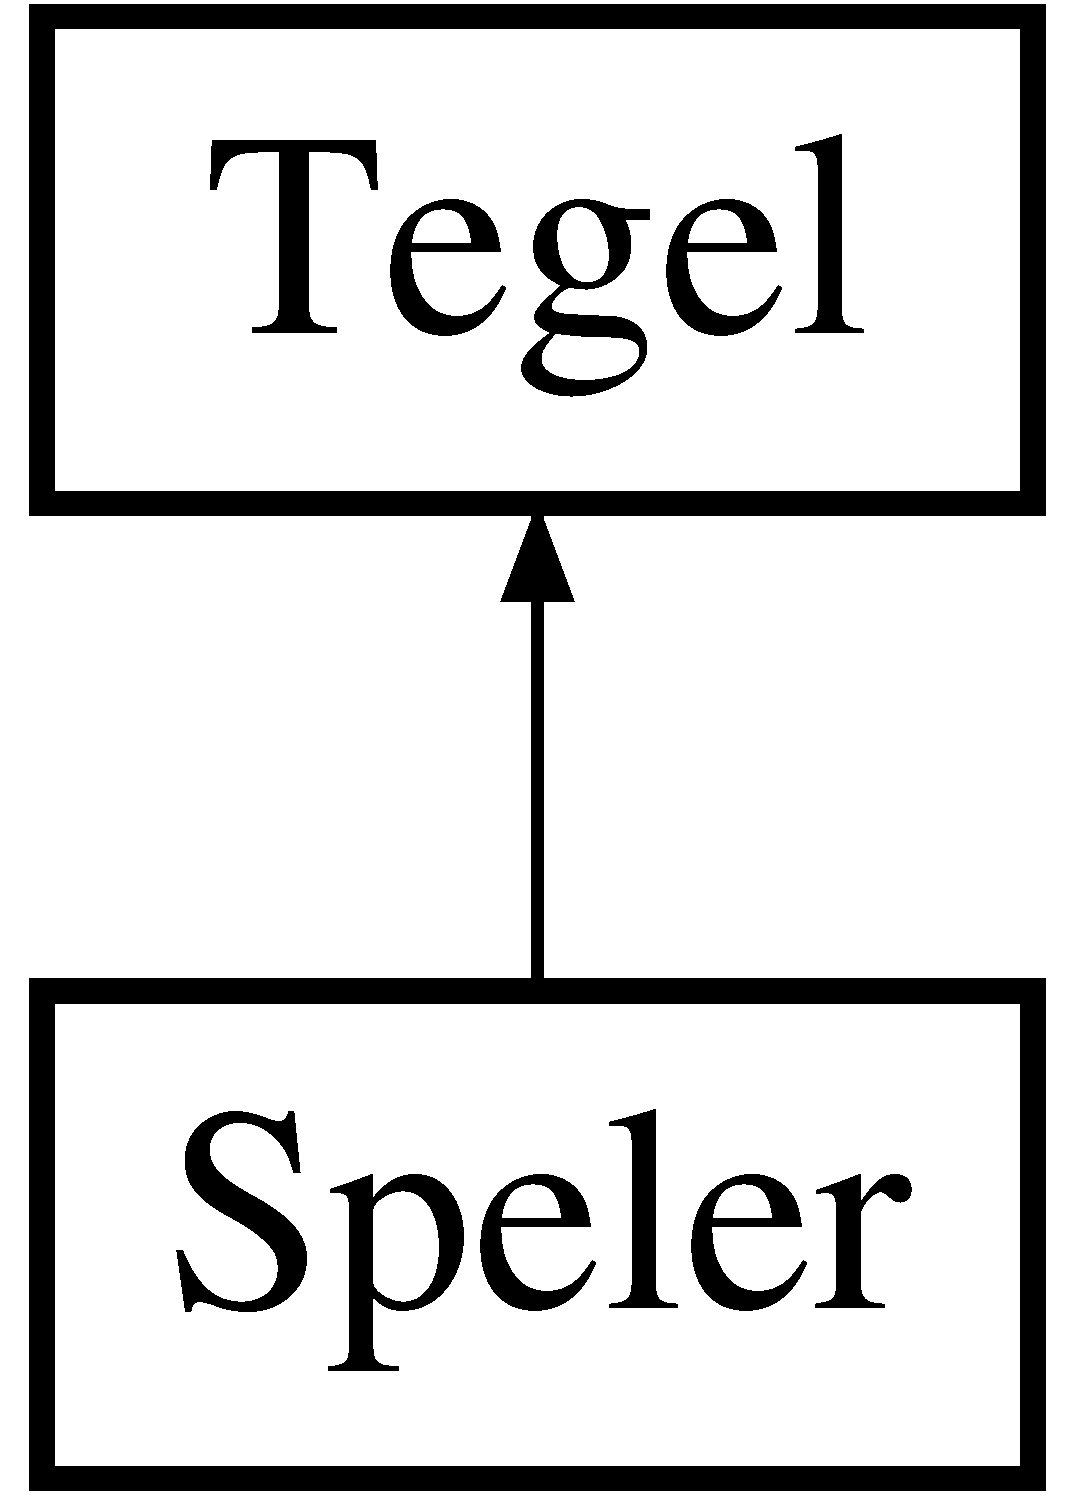
\includegraphics[height=2.000000cm]{class_speler}
\end{center}
\end{figure}
\subsection*{Public Member Functions}
\begin{DoxyCompactItemize}
\item 
\hyperlink{class_speler_af23b7a6a0b542e5a2a2f51be5d6bb043}{Speler} (int x, int y)
\item 
int \hyperlink{class_speler_abd8d3818f18cb18395b34484a4281ddf}{get\+Positie} ()
\item 
void \hyperlink{class_speler_a035f2db6c9ab98ee10e09f82576a5a2c}{update} (\hyperlink{classkey_manager}{key\+Manager} \hyperlink{classkey_manager}{key\+Manager})
\item 
void \hyperlink{class_speler_a93720a1aa0fe2bfee93c16aaf670894d}{render} (Graphics g, Buffer\+Strategy bs)
\item 
\hyperlink{enum_richting}{Richting} \hyperlink{class_speler_a35bd3987229c02b587c3dc53e90f97c0}{get\+Richting} (\hyperlink{classkey_manager}{key\+Manager} \hyperlink{classkey_manager}{key\+Manager})
\end{DoxyCompactItemize}
\subsection*{Additional Inherited Members}


\subsection{Detailed Description}
\begin{DoxyAuthor}{Author}
Kelvin 

Senne 

Corn� 

Jordy 

Aran
\end{DoxyAuthor}
\begin{DoxyVersion}{Version}
1.\+1 03/6/2017 
\end{DoxyVersion}
\begin{DoxySince}{Since}
1.\+0
\end{DoxySince}
This class creates the player 

\subsection{Constructor \& Destructor Documentation}
\mbox{\Hypertarget{class_speler_af23b7a6a0b542e5a2a2f51be5d6bb043}\label{class_speler_af23b7a6a0b542e5a2a2f51be5d6bb043}} 
\index{Speler@{Speler}!Speler@{Speler}}
\index{Speler@{Speler}!Speler@{Speler}}
\subsubsection{\texorpdfstring{Speler()}{Speler()}}
{\footnotesize\ttfamily Speler.\+Speler (\begin{DoxyParamCaption}\item[{int}]{x,  }\item[{int}]{y }\end{DoxyParamCaption})}

Constructor takes the x and y, and give this to \hyperlink{class_tegel}{Tegel} constructor with \char`\"{}super()\char`\"{} 
\begin{DoxyParams}{Parameters}
{\em x} & ; Used for the horizontal position \\
\hline
{\em y} & ; Used for the vertical position \\
\hline
\end{DoxyParams}
\begin{DoxySeeAlso}{See also}
\hyperlink{class_tegel}{Tegel} Constructor 
\end{DoxySeeAlso}


\subsection{Member Function Documentation}
\mbox{\Hypertarget{class_speler_abd8d3818f18cb18395b34484a4281ddf}\label{class_speler_abd8d3818f18cb18395b34484a4281ddf}} 
\index{Speler@{Speler}!get\+Positie@{get\+Positie}}
\index{get\+Positie@{get\+Positie}!Speler@{Speler}}
\subsubsection{\texorpdfstring{get\+Positie()}{getPositie()}}
{\footnotesize\ttfamily int Speler.\+get\+Positie (\begin{DoxyParamCaption}{ }\end{DoxyParamCaption})}

This method does nothing \mbox{\Hypertarget{class_speler_a35bd3987229c02b587c3dc53e90f97c0}\label{class_speler_a35bd3987229c02b587c3dc53e90f97c0}} 
\index{Speler@{Speler}!get\+Richting@{get\+Richting}}
\index{get\+Richting@{get\+Richting}!Speler@{Speler}}
\subsubsection{\texorpdfstring{get\+Richting()}{getRichting()}}
{\footnotesize\ttfamily \hyperlink{enum_richting}{Richting} Speler.\+get\+Richting (\begin{DoxyParamCaption}\item[{\hyperlink{classkey_manager}{key\+Manager}}]{key\+Manager }\end{DoxyParamCaption})}

This class renders the player. 
\begin{DoxyParams}{Parameters}
{\em \hyperlink{classkey_manager}{key\+Manager}} & ; Listen to key \\
\hline
\end{DoxyParams}
\begin{DoxyReturn}{Returns}
\hyperlink{enum_richting}{Richting} ; can be N\+O\+R\+TH, W\+E\+ST, E\+A\+ST or S\+O\+U\+TH
\end{DoxyReturn}
This method is used to check the neighbourfield in \hyperlink{class_speelveld}{Speelveld}. \mbox{\Hypertarget{class_speler_a93720a1aa0fe2bfee93c16aaf670894d}\label{class_speler_a93720a1aa0fe2bfee93c16aaf670894d}} 
\index{Speler@{Speler}!render@{render}}
\index{render@{render}!Speler@{Speler}}
\subsubsection{\texorpdfstring{render()}{render()}}
{\footnotesize\ttfamily void Speler.\+render (\begin{DoxyParamCaption}\item[{Graphics}]{g,  }\item[{Buffer\+Strategy}]{bs }\end{DoxyParamCaption})}

This method renders the player. 
\begin{DoxyParams}{Parameters}
{\em g} & ; Used for the Graphics \\
\hline
{\em bs;} & Used for the bufferstrategy\\
\hline
\end{DoxyParams}
It uses the \hyperlink{class_assets}{Assets} class and the positions to draw himself. This method is used by the 2d array from tiles in \hyperlink{class_speelveld}{Speelveld}. \mbox{\Hypertarget{class_speler_a035f2db6c9ab98ee10e09f82576a5a2c}\label{class_speler_a035f2db6c9ab98ee10e09f82576a5a2c}} 
\index{Speler@{Speler}!update@{update}}
\index{update@{update}!Speler@{Speler}}
\subsubsection{\texorpdfstring{update()}{update()}}
{\footnotesize\ttfamily void Speler.\+update (\begin{DoxyParamCaption}\item[{\hyperlink{classkey_manager}{key\+Manager}}]{key\+Manager }\end{DoxyParamCaption})}

This method updates the position of the player when a key is pressed 
\begin{DoxyParams}{Parameters}
{\em key\+Manger} & ; Listen to key\\
\hline
\end{DoxyParams}
If key\+Manger is true, position can be changed, otherwise it will move on an on. Then it will check which key was pressed. It uses Set\+XY from the positie class, this one takes the direction from the enum \hyperlink{enum_richting}{Richting}. \begin{DoxySeeAlso}{See also}
\hyperlink{class_tegel_a2a70fa00c15beb627f6f34ea8436d3df}{positie} 

\hyperlink{enum_richting}{Richting} 

\hyperlink{classkey_manager}{key\+Manager} 
\end{DoxySeeAlso}


The documentation for this class was generated from the following file\+:\begin{DoxyCompactItemize}
\item 
D\+:/users/senne/workspace/\+No\+Game/src/Speler.\+java\end{DoxyCompactItemize}

\hypertarget{class_tegel}{}\section{Tegel Class Reference}
\label{class_tegel}\index{Tegel@{Tegel}}
Inheritance diagram for Tegel\+:\begin{figure}[H]
\begin{center}
\leavevmode
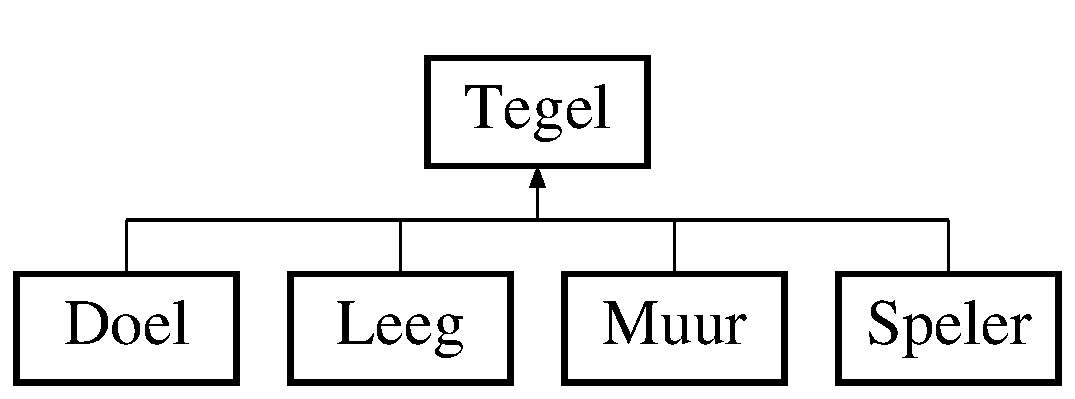
\includegraphics[height=2.000000cm]{class_tegel}
\end{center}
\end{figure}
\subsection*{Public Member Functions}
\begin{DoxyCompactItemize}
\item 
\hyperlink{class_tegel_a269c76f2f28b725bc720ee98b192371f}{Tegel} (int x, int y)
\item 
abstract int \hyperlink{class_tegel_a1a7dda59e0cd949366ca53890963a555}{get\+Positie} ()
\item 
abstract void \hyperlink{class_tegel_abc7f5173d69e3737da3496def320a2ec}{update} (\hyperlink{classkey_manager}{key\+Manager} \hyperlink{classkey_manager}{key\+Manager})
\item 
abstract void \hyperlink{class_tegel_a23f87e96ef260e41b2f16b8838c8fdac}{render} (Graphics g, Buffer\+Strategy bs)
\end{DoxyCompactItemize}
\subsection*{Protected Attributes}
\begin{DoxyCompactItemize}
\item 
\hyperlink{class_locatie}{Locatie} \hyperlink{class_tegel_a2a70fa00c15beb627f6f34ea8436d3df}{positie}
\end{DoxyCompactItemize}


\subsection{Detailed Description}
\begin{DoxyAuthor}{Author}
Kelvin 

Senne 

Corn� 

Jordy 

Aran
\end{DoxyAuthor}
\begin{DoxyVersion}{Version}
1.\+1 03/6/2017 
\end{DoxyVersion}
\begin{DoxySince}{Since}
1.\+0
\end{DoxySince}
This abstract class creates the tiles, these tiles can be\+: player, goal, empty or a wall. Moreover, \hyperlink{class_tegel}{Tegel} is used by \hyperlink{class_speelveld}{Speelveld} 

\subsection{Constructor \& Destructor Documentation}
\mbox{\Hypertarget{class_tegel_a269c76f2f28b725bc720ee98b192371f}\label{class_tegel_a269c76f2f28b725bc720ee98b192371f}} 
\index{Tegel@{Tegel}!Tegel@{Tegel}}
\index{Tegel@{Tegel}!Tegel@{Tegel}}
\subsubsection{\texorpdfstring{Tegel()}{Tegel()}}
{\footnotesize\ttfamily Tegel.\+Tegel (\begin{DoxyParamCaption}\item[{int}]{x,  }\item[{int}]{y }\end{DoxyParamCaption})}

A constructor. The constructor inits the place from the tiles. These tiles can be the following objects\+: player, goal, empty or a wall. 
\begin{DoxyParams}{Parameters}
{\em x} & ; Used for the horizontal position \\
\hline
{\em y} & ; Used for the vertical position \\
\hline
\end{DoxyParams}
\begin{DoxySeeAlso}{See also}
\hyperlink{class_speler}{Speler} 

\hyperlink{class_doel}{Doel} 

\hyperlink{class_muur}{Muur} 

\hyperlink{class_leeg}{Leeg} 
\end{DoxySeeAlso}


\subsection{Member Function Documentation}
\mbox{\Hypertarget{class_tegel_a1a7dda59e0cd949366ca53890963a555}\label{class_tegel_a1a7dda59e0cd949366ca53890963a555}} 
\index{Tegel@{Tegel}!get\+Positie@{get\+Positie}}
\index{get\+Positie@{get\+Positie}!Tegel@{Tegel}}
\subsubsection{\texorpdfstring{get\+Positie()}{getPositie()}}
{\footnotesize\ttfamily abstract int Tegel.\+get\+Positie (\begin{DoxyParamCaption}{ }\end{DoxyParamCaption})\hspace{0.3cm}{\ttfamily [abstract]}}

This method is abstract. ~\newline
 for more detailed description\+: ~\newline
 \begin{DoxySeeAlso}{See also}
\hyperlink{class_speler}{Speler} 

\hyperlink{class_doel}{Doel} 

\hyperlink{class_muur}{Muur} 

\hyperlink{class_leeg}{Leeg} 
\end{DoxySeeAlso}
\mbox{\Hypertarget{class_tegel_a23f87e96ef260e41b2f16b8838c8fdac}\label{class_tegel_a23f87e96ef260e41b2f16b8838c8fdac}} 
\index{Tegel@{Tegel}!render@{render}}
\index{render@{render}!Tegel@{Tegel}}
\subsubsection{\texorpdfstring{render()}{render()}}
{\footnotesize\ttfamily abstract void Tegel.\+render (\begin{DoxyParamCaption}\item[{Graphics}]{g,  }\item[{Buffer\+Strategy}]{bs }\end{DoxyParamCaption})\hspace{0.3cm}{\ttfamily [abstract]}}

This method is abstract for more detailed description \begin{DoxySeeAlso}{See also}
\hyperlink{class_speler}{Speler} 

\hyperlink{class_doel}{Doel} 

\hyperlink{class_muur}{Muur} 

\hyperlink{class_leeg}{Leeg} for more detailed description 
\end{DoxySeeAlso}
\mbox{\Hypertarget{class_tegel_abc7f5173d69e3737da3496def320a2ec}\label{class_tegel_abc7f5173d69e3737da3496def320a2ec}} 
\index{Tegel@{Tegel}!update@{update}}
\index{update@{update}!Tegel@{Tegel}}
\subsubsection{\texorpdfstring{update()}{update()}}
{\footnotesize\ttfamily abstract void Tegel.\+update (\begin{DoxyParamCaption}\item[{\hyperlink{classkey_manager}{key\+Manager}}]{key\+Manager }\end{DoxyParamCaption})\hspace{0.3cm}{\ttfamily [abstract]}}

This method is abstract for more detailed description \begin{DoxySeeAlso}{See also}
\hyperlink{class_speler}{Speler} 

\hyperlink{class_doel}{Doel} 

\hyperlink{class_muur}{Muur} 

\hyperlink{class_leeg}{Leeg} 
\end{DoxySeeAlso}


\subsection{Member Data Documentation}
\mbox{\Hypertarget{class_tegel_a2a70fa00c15beb627f6f34ea8436d3df}\label{class_tegel_a2a70fa00c15beb627f6f34ea8436d3df}} 
\index{Tegel@{Tegel}!positie@{positie}}
\index{positie@{positie}!Tegel@{Tegel}}
\subsubsection{\texorpdfstring{positie}{positie}}
{\footnotesize\ttfamily \hyperlink{class_locatie}{Locatie} Tegel.\+positie\hspace{0.3cm}{\ttfamily [protected]}}

positie is used for location 

The documentation for this class was generated from the following file\+:\begin{DoxyCompactItemize}
\item 
D\+:/users/senne/workspace/\+No\+Game/src/Tegel.\+java\end{DoxyCompactItemize}

%--- End generated contents ---

% Index
\backmatter
\newpage
\phantomsection
\clearemptydoublepage
\addcontentsline{toc}{chapter}{Index}
\printindex

\end{document}
